\documentclass[tikz,border=2pt]{standalone}
\usepackage{amsmath}
\usepackage{amssymb}
\usepackage{xcolor}

\definecolor{journalink}{HTML}{1F1C18}
\definecolor{journalmuted}{HTML}{8A7F72}
\definecolor{journalaccent}{HTML}{9C2D2D}

\begin{document}
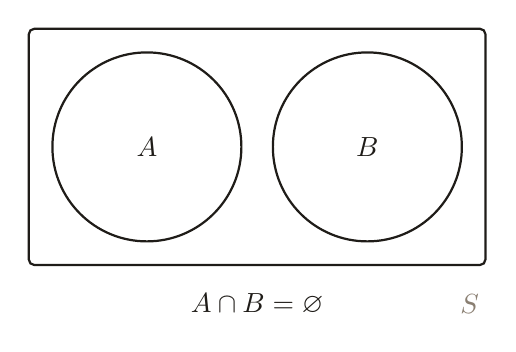
\begin{tikzpicture}[x=1cm, y=1cm, every node/.style={font=\normalsize}]

  \draw[journalink, line width=0.8pt, rounded corners=2pt] (-1.5,-1.5) rectangle (4.3,1.5);
  \draw[journalink, line width=0.8pt] (0,0) circle (1.2);
  \draw[journalink, line width=0.8pt] (2.8,0) circle (1.2);
  \node[journalink] at (0,0) {$A$};
  \node[journalink] at (2.8,0) {$B$};
  \node[journalink] at (1.4,-2.0) {$A\cap B=\varnothing$};
  \node[journalmuted] at (4.1,-2.0) {$S$};

\end{tikzpicture}
\end{document}
